\section{Transparencia Inducida Electromagnéticamente (EIT) en celdas de vapores alcalinos: fundamentos teóricos y aplicaciones espectroscópicas}
\subsection{Motivación para la elección del tema}
\subsubsection{La Transparencia Inducida Electromagnéticamente (EIT)}
La Transparencia Inducida Electromagnéticamente (EIT) es un fenómeno de óptica cuántica no lineal donde un medio atómico originalmente opaco se vuelve transparente a una frecuencia de transición específica debido a la presencia de un campo láser auxiliar.

En condiciones habituales, un haz láser de prueba (probe) ajustado a la frecuencia de resonancia de un átomo es fuertemente absorbido. Sin embargo, cuando se aplica simultáneamente un segundo haz de acoplamiento (coupling) más intenso que interactúa con un estado atómico contiguo, se genera una interferencia cuántica destructiva entre las amplitudes de transición óptica. Esta interferencia anula la absorción y abre una "ventana" de transparencia extremadamente estrecha en el centro del perfil espectral.

\begin{figure}
    \centering
    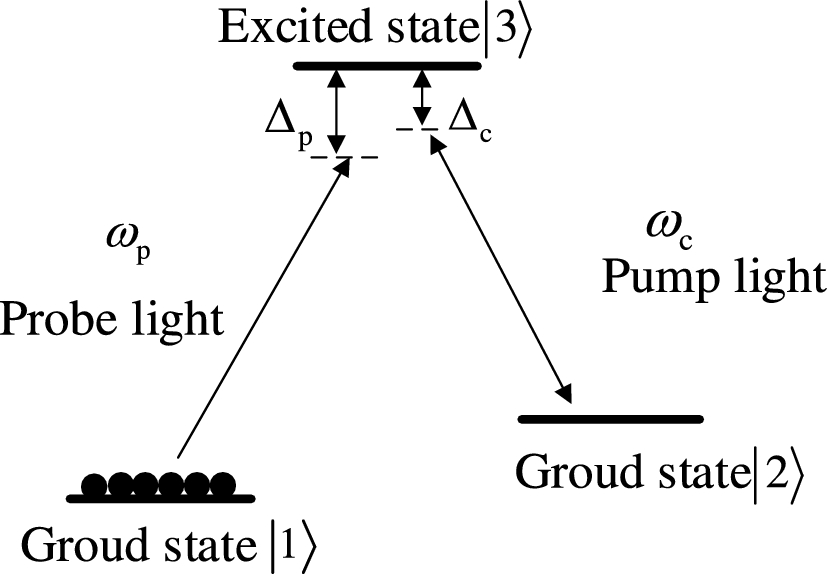
\includegraphics[width=0.7\textwidth]{figures/EIT_diagram.png}
    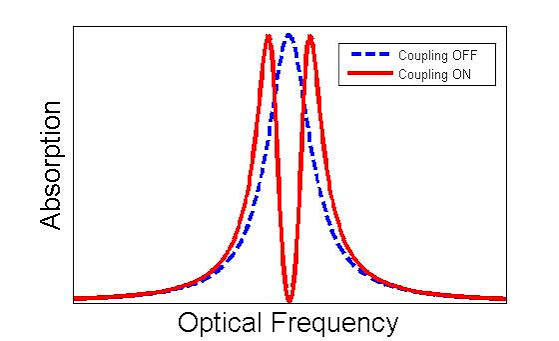
\includegraphics[width=0.7\textwidth]{figures/EIT_spectrum.jpg}
\end{figure}
\subsubsection{Motivación}
\begin{enumerate}
    \item \textbf{Rigor Teórico y Física Atómica Cuántica:} La EIT representa uno de los fenómenos más paradigmáticos de la óptica cuántica y la física atómica de multinivel. Su estudio exige superar los modelos semiclásicos simplificados de dos niveles para adentrarse en la coherencia cuántica y la interferencia destructiva de amplitudes de transición en sistemas de tres o más niveles.
    \item \textbf{Sinergia Directa con el Proyecto de Tesis (Ajuste de Espectros en Vapores Alcalinos):} Actualmente desarrollo mi trabajo de tesis centrado en el diseño de software para el ajuste de espectros de absorción en celdas de vapores alcalinos. En experimentos reales con campos de radiación intensos, la absorción no se comporta como una simple envolvente Voigt o Lorentziana. La presencia de coherencias atómicas modifica drásticamente la susceptibilidad eléctrica compleja, generando estrechas ventanas de transparencia y dispersiones extremadamente anómalas. El desarrollo de esta monografía aporta el sustento teórico indispensable para parametrizar correctamente las formas de línea (line shapes) en algoritmos numéricos de ajuste espectroscópico.
    \item \textbf{Relevancia Tecnológica:}Las celdas de vapor atómico caliente constituyen la plataforma fundamental para la implementación práctica de EIT. Este fenómeno es el mecanismo físico subyacente en aplicaciones de vanguardia como la reducción drástica de la velocidad de grupo de la luz (luz lenta y luz almacenada), el desarrollo de memorias cuánticas atómicas y la metrología/magnetometría de alta sensibilidad.
\end{enumerate}
\subsection{Posibles aplicaciones y relaciones con la física atómica y molecular}
Manipulación de la velocidad de grupo de la luz (luz lenta y almacenada), metrología cuántica, magnetometría de alta sensibilidad y el desarrollo de memorias cuánticas en celdas térmicas de vapor.
\subsection{Objetivos}
Realizar una revisión analítica y formal de los fundamentos teóricos, la descripción mediante el formalismo de la matriz de densidad y las implicaciones espectroscópicas de la Transparencia Inducida Electromagnéticamente (EIT) en celdas de vapores alcalinos, estableciendo la relación entre los parámetros de coherencia cuántica y el modelado preciso de perfiles de absorción para su uso en espectroscopía de alta resolución.

\subsubsection{Objetivos específicos}
\begin{itemize}
    \item \textbf{Desarrollar el formalismo matemático básico:} Deducir, a partir de la ecuación de Liouville-von Neumann bajo la Aproximación de Onda Giratoria (RWA), las ecuaciones de movimiento para las componentes de la matriz de densidad ($\rho$) en un sistema de 3 niveles en configuración $\Lambda$.
    \item \textbf{Obtener las propiedades ópticas del medio:} Derivar la expresión analítica de la susceptibilidad eléctrica coherente $\chi(\omega)$ para analizar en detalle la cancelación de la componente imaginaria ($\chi''$, absorción) en la condición de resonancia de dos fotones.
    \item \textbf{Evaluar los efectos reales en celdas térmicas:} Analizar el impacto de las condiciones experimentales en celdas de vapores alcalinos incluyendo el ensanchamiento Doppler, el bombeo óptico en la estructura hiperfina y las tasas de descoherencia por tiempo de tránsito o colisiones.
    \item \textbf{Estudiar la respuesta espectroscópica para el ajuste numérico:} Comparar las diferencias entre perfiles simétricos tradicionales (Lorentz/Voigt) y las ventanas de transparencia coherentes (perfiles EIT/Fano), identificando las variables físicas críticas que deben parametrizarse en algoritmos de ajuste de curvas.
    \item \textbf{Mostrar las aplicaciones principales:} Documentar brevemente las implicaciones del control de la velocidad de grupo y su uso en almacenamiento de fotones y metrología cuántica.
\end{itemize}
\subsection{Metas para la primera mitad del semestre}
Haber desarrollado el formalismo matemático básico y haber obtenido las propiedades ópticas del medio, incluyendo la derivación de la susceptibilidad eléctrica coherente $\chi(\omega)$ y la identificación de los parámetros críticos para el modelado de perfiles de absorción en condiciones experimentales realistas.
\nocite{*}